\documentclass[a4paper, 14pt]{extarticle}

\usepackage{ifluatex}
\usepackage{ifpdf}

\ifluatex
\usepackage{fontspec}
\defaultfontfeatures{Renderer=Basic,Ligatures={TeX}}
\setmainfont{CMU Serif}
\setsansfont{CMU Sans Serif}
\usepackage{polyglossia}
\setdefaultlanguage{russian}
\setotherlanguage{english}
\setmainfont{CMU Serif}
\newfontfamily{\cyrillicfont}{CMU Serif}
\setsansfont{CMU Sans Serif}
\newfontfamily{\cyrillicfontsf}{CMU Sans Serif}
\setmonofont{CMU Typewriter Text}
\newfontfamily{\cyrillicfonttt}{CMU Typewriter Text}
\else
\ifpdf 
\usepackage[T2A]{fontenc}
\usepackage[utf8]{inputenc}
\usepackage[english,russian]{babel}
\typeout{PDF only}
\fi
\fi

\usepackage[left=1cm,right=1cm,top=2cm,bottom=2cm]{geometry}
%%% Дополнительная работа с математикой
\usepackage{amsfonts,amssymb,amsthm,mathtools} % AMS
\usepackage{amsmath}
\usepackage{icomma} % «Умная» запятая: $0,2$ — число, $0, 2$ — перечисление

\usepackage{mathrsfs} % Красивый матшрифт

%% Перенос знаков в формулах (по Львовскому)
\newcommand*{\hm}[1]{#1\nobreak\discretionary{}
  {\hbox{$\mathsurround=0pt #1$}}{}}

%%% Работа с картинками

\usepackage{graphicx}  % Для вставки рисунков
\graphicspath{ {images/} }
\setlength\fboxsep{3pt} % Отступ рамки \fbox{} от рисунка
\setlength\fboxrule{1pt} % Толщина линий рамки \fbox{}
\usepackage{wrapfig} % Обтекание рисунков и таблиц текстом

\usepackage[dvipsnames]{xcolor}
\usepackage{verbatim}
\usepackage{hyperref}

\usepackage{listings}

\lstdefinelanguage{JavaScript}{
  keywords={let, typeof, new, true, false, catch, function, return, null, catch, switch, var, if, in, while, do, else, case, break, const},
  keywordstyle=\color{blue}\bfseries,
  ndkeywords={class, export, boolean, throw, implements, import, this,},
  ndkeywordstyle=\color{darkgray}\bfseries,
  identifierstyle=\color{black},
  sensitive=false,
  comment=[l]{//},
  morecomment=[s]{/*}{*/},
  commentstyle=\color{green}\ttfamily,
  stringstyle=\color{red}\ttfamily,
  morestring=[b]',
  morestring=[b]",
  escapechar=|
}

\lstset{
  language=JavaScript,
  extendedchars=true,
  basicstyle=\small\ttfamily,
  showstringspaces=false,
  breakatwhitespace=true,
  showspaces=false,
  numbers=left,
  numberstyle=\footnotesize,
  numbersep=9pt,
  tabsize=2,
  keepspaces=true,
  breaklines=true,
  showtabs=false,
  captionpos=b
  escapechar=|,
  frame=single ,
  commentstyle=\itshape ,
  frameshape={RYR}{Y}{Y}{RYR},
  stringstyle =\bfseries,
}

\usepackage{autobreak}

\newcommand*{\function}[2]{\texttt{\textcolor{Red}{function} \textcolor{Purple}{#1}(#2)}\linebreak}

\newcommand*{\prototype}[3][]{\texttt{\textcolor{Orange}{#2}.\textcolor{Blue}{prototype}.\textcolor{Purple}{#3} = \textcolor{Red}{function}(#1)}\linebreak}

\usepackage{titlesec}

\setcounter{secnumdepth}{4}

\titleformat{\paragraph}
{\normalfont\normalsize\bfseries}{\theparagraph}{1em}{}
\titlespacing*{\paragraph}
{0pt}{3.25ex plus 1ex minus .2ex}{1.5ex plus .2ex}

\usepackage{multicol}
\setlength{\columnsep}{1cm}

\usepackage[most]{tcolorbox}

\newtcolorbox{leftBox}{
  colback=white,colframe=black, 
  width = 0.97\linewidth,
  sharp corners = southwest,
}

\usepackage{newfloat,caption,float}
\usepackage{capt-of}

\DeclareFloatingEnvironment[
  fileext = loe,
  listname = Задача,
  name = Задача.,
  placement = H,
  within = none,
  ]{application}
\captionsetup[application]{labelfont=md}

\DeclareFloatingEnvironment[
  fileext = loe,
  listname = Рис,
  name = Рис.,
  placement = H,
  within = none,
  ]{image}
\captionsetup[image]{labelfont=md}

\usepackage{tikz,tikz-3dplot}

\renewcommand{\lstlistingname}{Листинг}% Listing -> Листинг


\newcommand*{\task}[4]{
  \begin{minipage}[t]{\linewidth}
  \begin{multicols}{2}
    #1\\\\
    Ответ: $#2$\\
    \includegraphics[width=0.4\textwidth]{#3}
  \end{multicols}
  \captionof{application}{Пример генерации задания с помощью #4}
\end{minipage}
}
\renewcommand{\baselinestretch}{1.37}

\begin{document}


\begin{center}
	\hfill \break
	\large{МИНОБРНАУКИ РОССИИ}\\
	\footnotesize{ФЕДЕРАЛЬНОЕ ГОСУДАРСТВЕННОЕ БЮДЖЕТНОЕ ОБРАЗОВАТЕЛЬНОЕ УЧРЕЖДЕНИЕ}\\
	\footnotesize{ВЫСШЕГО ПРОФЕССИОНАЛЬНОГО ОБРАЗОВАНИЯ}\\
	\small{\textbf{«ВОРОНЕЖСКИЙ ГОСУДАРСТВЕННЫЙ УНИВЕРСИТЕТ»}}\\
	\hfill \break
	\normalsize{Математический факультет}\\
	\hfill \break
	\normalsize{Кафедра теории функций и геометрии}\\
	\hfill\break
	\hfill \break
	\hfill \break
	\hfill \break
	\large{Программная реализация (на языке JavaScript) алгоритмов генерации ФОС ЕГЭ по геометрии в 2024 году}\\
	\hfill \break
	\hfill \break
	\hfill \break
	\hfill \break
	\hfill \break
	\normalsize{Курсовая работа\\
		\hfill \break
		Направление  010501 Фундаментальные математика и механика\\

		\hfill \break
	}\\
	\hfill \break
	\hfill \break
\end{center}
\hfill \break

\normalsize{
	\begin{tabular}{cccc}
		Зав.кафедрой & \underline{\hspace{3cm}} & д.физ.-мат.н.,  проф. & Е.М. Семёнов    \\\\
		Обучающийся  & \underline{\hspace{3cm}} &                       & А.С. Суматохина \\\\
		Руководитель & \underline{\hspace{3cm}} & д.физ.-мат.н.,  проф. & Е.М. Семёнов    \\\\
	\end{tabular}
}\\
\hfill \break
\hfill \break
\begin{center} Воронеж 2024 \end{center}
\thispagestyle{empty} % выключаем отображение номера для этой страницы

% КОНЕЦ ТИТУЛЬНОГО ЛИСТА


\tableofcontents


\section*{Введение}
\addcontentsline{toc}{section}{Введение}
Единый государственный экзамен (ЕГЭ)~— централизованно проводимый в Российской
Федерации экзамен в средних учебных заведениях — школах, лицеях и гимназиях,
форма проведения ГИА (Государственной Итоговой Аттестации) по образовательным программам среднего общего образования.
Служит одновременно выпускным экзаменом из школы и вступительным экзаменом в вузы.

Но за время обучения в 10 и 11 классе при подготовке к ЕГЭ школьники сталкиваются с дефицитом заданий по определённым категориям.
Так, в конце 2021 года в список заданий ЕГЭ были добавлены новые задания под номером 11 по теме «Графики функций», а в конце 2023 — задание №2 по теме «Векторы», количество которых для прорешивания было очень мало. 
А по теме «Производная и первообразная» банк заданий расходуется при подготовке с невероятной скоростью:
так как это преимущественно графические задания, решение их занимает менее минуты, а их составление вручную занимает несоразмерно много времени.ЕГЭ является относительно неизменяемым экзаменом, поэтому все материалы, которые уже были выложены в открытый доступ, имеют полные решения, что приводит к списыванию учениками.

При этом существуют задания со вспомогательным чертежом. Чаще всего для целого ряда заданий используется одна и та же иллюстрация, которая не всегда соответствуют условиям задачи, а иногда отвлекает от решения.
Проект «Час ЕГЭ» позволяет решить все эти проблемы.

«Час ЕГЭ» — компьютерный образовательный проект, разрабатываемый при математическом
факультете ВГУ в рамках «OpenSource кластера» и предназначенный для помощи учащимся
старших классов при подготовке к тестовой части единого государственного экзамена.
%%ссылочки на доклады
Задания в «Час ЕГЭ» генерируются случайным образом по специализированным алгоритмам,
называемых шаблонами, каждый из которых
охватывает множество вариантов соответствующей ему задачи. Для
пользователей
предназначены четыре оболочки (режима работы): «Случайное задание», «Тесты на печать»,
«Полный тест» и «Мини-интеграция».
«Час ЕГЭ» является полностью открытым (код находится под лицензией GNU GPL 3.0)
и бесплатным.
В настоящее время в проекте полностью реализованы тесты по математике с кратким
ответом (бывшая «часть В»).~\cite{fipi}
Планируется с течением времени включить в проект тесты по другим предметам школьной
программы.

Первая глава этой работы посвящена обзору вспомогательных функций, которые ускоряют написание шаблонов по теме «Планиметрия» и введению в проект элементов декларативного программирования. Также приведён алгоритм написания шаблона с чертежом.

Вторая глава представляет решение проблемы отрисовки фигур в трёхмерном пространстве на языке программирования JavaScript; рассказывает о применении объектно-ориентированного программирования для упрощения написания шаблонов с чертежом; затрагивает вопрос об написании программного кода при помощи нейросетей; приводит обзор вспомогательных функций и алгоритм написания шаблона по теме «Стереометрия». 


%Цели
%всп функции для иллюстрирования
%шаблоны

%Задачи
%всп функции для иллюстрирования
%классы для 
%шаблоны



%%Программная реализация (на языке Javascript) алгоритмов
%% генерации фонда оценочных средств по математике
\section{Планиметрия}
В это главе мы приводим вспомогательные функции и алгоритм написания шаблона по планиметрии
\subsection{Вспомогательные функции}
\subsubsection{Функции для работы с массивами}
\prototype[repeat]{Array}{permuteCyclic}
Возвращает массив после циклической перестановки.
В листинге \ref{lst:92} в строке \ref{line:permuteCyclic-1} функция используется для перестановки букв в названии параллелограмма, а в строке \ref{line:permuteCyclic-2} — в названии трапеции.

\begin{lstlisting}
    let array = [1, 2, 3, 4, 5];

    array.permuteCyclic(1);
    // [5, 1, 2, 3, 4]

    array.permuteCyclic(-2);
    // [3, 4, 5, 1, 2]

    array.permuteCyclic(0);
    // [1, 2, 3, 4, 5]
    \end{lstlisting}

\prototype{Array}{mt\_coordinatesOfIntersectionOfTwoSegments\\}
Возвращает координаты пересечения двух отрезков, задаваемых первыми парами точек из массива. Является вспомогательной для функции \texttt{arcBetweenSegments}.

\begin{lstlisting}[escapechar=|]
    let array = [{x:0,y:5},{x:-4,y:4},{x:1,y:10},{x:-3,y:6}];

    array.mt_coordinatesOfIntersectionOfTwoSegments()
    //{ x: -5.333333333333333, y: 3.666666666666667, status: false }
    //Если status — false, отрезки не пересекаются, но прямые проходящие через них пересекаются в точке {x,y}

    array = [{x:0,y:5},{x:-4,y:4},{x:1,y:1},{x:-3,y:6}];
    array.mt_coordinatesOfIntersectionOfTwoSegments()
    //{ x: -1.8333333333333333, y: 4.541666666666667, status: true }
    //Если status — true, отрезки пересекаются в точке {x,y}
        
\end{lstlisting}

\prototype[separator]{Array}{shuffleJoin}
Перемешивает и соединяет массив с разделителем \texttt{separator}. \texttt{separator} по умолчанию пустая строка. Функция используется в \ref{lst:3011}
в строке \ref{line:shuffleJoin} для отображения условий задачи в случайном порядке.

\begin{lstlisting}
    let array = ['A', 'B', 'C', 'D',];
    array.shuffleJoin();
    //ADBC

    array.shuffleJoin('; ');
    //C; D; B; A 
\end{lstlisting}

\prototype[separator]{Array}{joinWithConjunction}
Соединяет массив запятыми и соединяет два последних элемента союзом «и».

\begin{lstlisting}
    let array = ['A', 'B', 'C', 'D',];

    array.joinWithConjunction();
    //A, B, C и D
\end{lstlisting}

\subsubsection{Функции для работы с числами}
\prototype{Number}{perfectCubicMultiplier}
Возвращает максимальный делитель данного числа, куб которого также является делителем данного числа.

\begin{lstlisting}
    let number = 81;

    number.perfectCubicMultiplier()
    //3

    number = 36;
    number.perfectCubicMultiplier()
    //1

    number = -27;
    number.perfectCubicMultiplier()
    //3
\end{lstlisting}

\prototype[p1, p2]{Number}{texcbrt}
TeX-представление кубического корня из данного числа.\\
Если данное число - полный куб, то корень из числа.\\
Если \texttt{p1}, то из-под корня будут вынесены возможные множители.\\
Если \texttt{p1}, \texttt{p2} и из-под корня выносится единица, то она будет опущена\\

\includegraphics[width=0.8\textwidth]{texcbrt.png}

\subsubsection{Функции для работы с canvas}
\prototype[vertex,\\ fillStyle]{CanvasRenderingContext2D}{drawSection}
Заполняет область цветом \texttt{fillStyle} по вершинам из массива \texttt{vertex}.

\begin{lstlisting}
    let paint1 = function(ctx) {
        let h = 400;
        let w = 400;
        ctx.drawCoordinatePlane(w, h, {
            hor: 1,
            ver: 1
        }, {
            x1: '1',
            y1: '1',
            sh1: 16,
        },30);
        ctx.scale(30, -30);
        ctx.drawSection([[1, 3],[-3, 0],[-2, -2],[1, -1],[5, 1],[4, 4],[3, 2]]);

        ctx.drawSection([[-2, 0],[-1, 1],[-4, 3],[-1, 5],[1, 1],[5, 2],[4, -6],[0, 0],[-4, -2],]);
    };
    \end{lstlisting}
    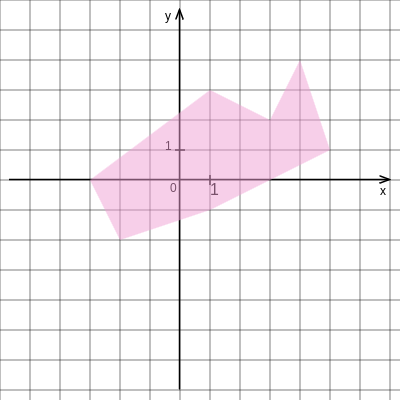
\includegraphics[width=0.4\textwidth]{drawSection-1.png}
    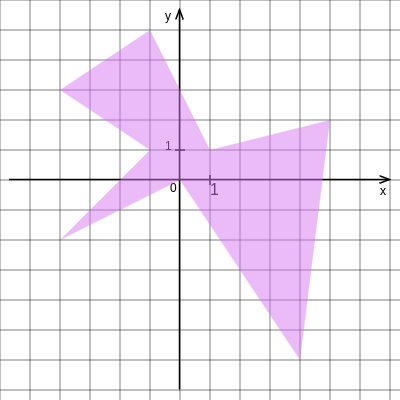
\includegraphics[width=0.4\textwidth]{drawSection-2.png}

\prototype[x, y,\\ angle, length]{CanvasRenderingContext2D}{drawLineAtAngle}
Рисует отрезок длины \texttt{length} под углом angle ( в радианах). Пример использования можно найти в листинге \ref{lst:2069} в строках \ref{line:drawLineAtAngle-1} и \ref{line:drawLineAtAngle-2} (применяется для отрисовки биссектрисы). 

\prototype[x1, y1, x2, y2, length, quantity]{CanvasRenderingContext2D}{strokeInMiddleOfSegment\\}
Ставит штрихи длины \texttt{length} на середине отрезка перпендикулярно ему. Функция используется в листинге \ref{lst:2069} в строках \ref{line:strokeInMiddleOfSegment-1}-\ref{line:strokeInMiddleOfSegment-2} для обозначения равных по длине сторон треугольника.

\prototype[x, y, angle, letter, length, maxLength]{CanvasRenderingContext2D}{markSegmentWithLetter\\}
Вспомогательная функция для отрисовки текста около некоторого отрезка.

\prototype[x1, y1, x2, y2, letter, length, maxLength]{CanvasRenderingContext2D}{signSegmentInMiddle\\}
Рисует строку \texttt{letter} на середине отрезка. В листинге \ref{lst:27193} в строках \ref{line:signSegmentInMiddle-1} - \ref{line:signSegmentInMiddle-2} функция используется для отображения длин рёбер многогранника.

\prototype[coordinates, radius]{CanvasRenderingContext2D}{arcBetweenSegments\\}
Рисует знак угла между двумя отрезками в месте их пересечения. \texttt{coordinates} - массив вида \texttt{[x1, y1, x2, y2]}.

\begin{lstlisting}
    let paint1 = function(ctx) {
        let h = 400;
        let w = 400;
        ctx.drawCoordinatePlane(w, h, {
            hor: 1,
            ver: 1
        }, {
            x1: '1',
            y1: '1',
            sh1: 16,
        }, 30);
        ctx.scale(30, -30);

        ctx.lineWidth = 2 / 30;
        ctx.drawLine(1, 5, 3, -2);
        ctx.drawLine(3, -2, 5, -3);
        ctx.arcBetweenSegments([1, 5, 3, -2, 5, -3], 2);

        ctx.drawLine(2, -5, -4, -2);
        ctx.drawLine(1, -2, -3, -6);
        ctx.arcBetweenSegments([2, -5, -4, -2,  -3, -6,1, -2,], 1);

        ctx.drawLine(1, 5, 1, -2);
		    ctx.drawLine(1, -2, 5, -2);
		    ctx.strokeStyle = om.secondaryBrandColors.iz();
		    ctx.arcBetweenSegments([1, 5, 1, -2, 5, -2], 3);

    };
\end{lstlisting}

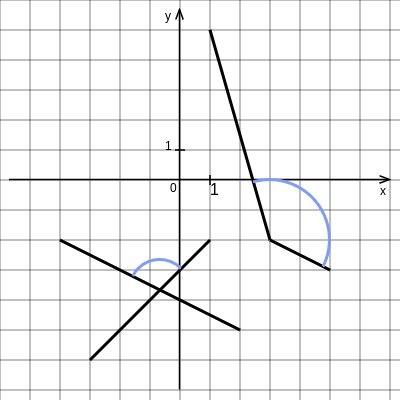
\includegraphics[width=0.4\textwidth]{arcBetweenSegments-1.png}    
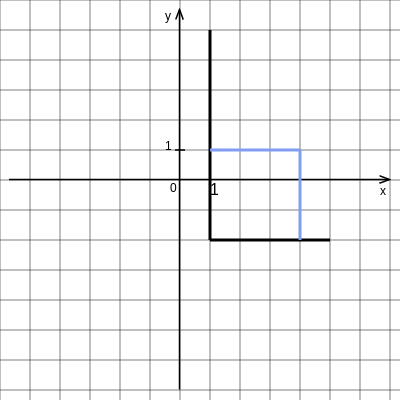
\includegraphics[width=0.4\textwidth]{arcBetweenSegments-2.png}    

\prototype[coordinates, radius, number, step]{CanvasRenderingContext2D}{arcBetweenSegmentsCount\\}
Рисует знак угла между двумя отрезками в месте их пересечения \texttt{number} раз с отступом \texttt{step}. В листинге \ref{lst:27764} в строках \ref{line:arcBetweenSegmentsCount-1} - \ref{line:arcBetweenSegmentsCount-2} используется для обозначения двух равных углов.

\prototype[x, y, radiusX, radiusY, rotation, startAngle, endAngle,\\ anticlockwise]{CanvasRenderingContext2D}{drawEllipse\\}
Рисует эллипс.

\prototype[x, y, radius, startAngle, endAngle, anticlockwise]{CanvasRenderingContext2D}{drawArc\\}
Рисует дугу.

\subsubsection{Элементы декларативного программирования}

\textbf{Определение.} Декларативное программирование — парадигма программирования, в которой задается спецификация решения задачи, то есть описывается конечный результат, а не способ его достижения.~\cite{posobie}

Во время разработки шаблонов по теме «Графики функции» требовалось много раз переопределять коэффициенты функций через циклы 
\texttt{while} или \texttt{do\dots while}, пока они не начнут соответствовать заданным условиям (видимость графика, сливание его с осями, видимость целых точек). Это часто приводило к бесконечной работе шаблона, при этом сложно было определить, какое условие не выполняется.

Для этого было разработано окружение \texttt{retryWhileUndefined} для шаблонов, которое бы перезапускало их не более \texttt{maxIterations} раз, если одно из условий не удовлетворено. 

\function{retryWhileUndefined}{theFunction, maxIterations}

Но всё равно было тяжело определить, почему шаблон перезапускается. Для этого было разработано более совершенное окружение \texttt{retryWhileError}, которое не только могло бы ограничивать количество перезапусков, но и фиксировать, какие проверки не были пройдены и выводить их на экран (ошибки видны только для разработчика при отладке).

\function{retryWhileError}{theFunction, maxIterations,maxCollectedErrors}

Для окружения были написаны функции-утверждения, которые имеют структуру : условие не выполнено - записать ошибку - перезапустить шаблон. Если максимальное количество повторений достигнуто, то вывести накопившиеся ошибки и количество их появлений. 

\function{genAssert}{condition, message}
    Если условие \texttt{condition} ложно, то шаблон перезапускается. 

\function{genAssertNonempty}{array, message}
    Если массив \texttt{array} пуст, то шаблон перезапускается.

\function{genAssertZ1000}{number, message}
    Если число \texttt{number} имеет более 3 знаков после запятой, то шаблон перезапускается.
    
\function{genAssertIrreducible}{numerator, denominator, message}
    Если дробь \texttt{numerator/denominator} сократима, то шаблон перезапускается.

\function{genAssertSaneDecomposition}{number, maxFactor, message}
    Если \texttt{number} число не раскладывается на простые множители, не более одного из которых превосходит \texttt{maxFactor}, то шаблон перезапускается. 

\subsection{Этапы разработки шаблона со вспомогательным чертежом по теме «Планиметрия»}

Для примера возьмём задание №19416~\cite{egemath}.
\\
\textbf{Задача №19376.}
В треугольнике $ABC$ известно, что ${AC=BC}$, $AB=16$, $AH$ — высота, $BH=4$. Найдите косинус угла $BAC$.\\ 

Заготовка шаблона имеет вид.

\lstinputlisting[]{code/109_1.js}

\begin{enumerate}
    \item Начнём с отрисовки чертежа для задания. Отметим стороны треугольника так, чтобы он лежал в центре холста, а до краёв оставалось 10-20px. При отрисовке используем функцию \texttt{drawLine}. Добавим высоту 
    \lstinputlisting[]{code/109_2.js} 
    \item Добавим на рисунок штрихи, указывающие на равенство сторон и обозначение прямого угла при помощи функций strokeInMiddleOfSegment и arcBetweenSegments соответственно. И подпишем вершины и точку перпендикуляра. Добавим модификатор \texttt{NAtask.modifiers.variativeABC(vertices)}, который заменяет все буквы в задании на случайные.
    %TODO: пояснить за параметр

    \lstinputlisting[]{code/109_3.js} 
    \item Теперь добавим ответ в задание. Проверим при помощи \texttt{genAssertZ1000}, что ответ имеет не более трёх знаков после запятой (если иначе шаблон запускается заново). Поместим все буквы и числа в \$\dots\$. Все условия из задачи преобразуем в массив и соединим случайным образом с помощью функции \texttt{shuffleJoin}.
    \lstinputlisting[]{code/109_4.js} 
\end{enumerate}



\section{Глава вторая}\label{2sect}
\subsection{Разработка библиотек с помощью Gpt-Chat}

На данный момент в языке JavaScript отсутствуют встроенные средства для изображения трёхмерных фигур. И существует только одна подходящая библиотека \texttt{Three.js}, которая могла бы выполнить проецирование координат фигуры на плоскость с учётом положения наблюдателя. Возможности библиотеки во много раз превосходят требуемую функциональность для нашего проекта.

Подобные ей библиотеки проводят проецирование на плоскость с поворотом только вокруг осей $OX$ и $OZ$. Что при отрисовке более сложных чертежей является недостаточным.

С учётом самых современных технологий, встал закономерный вопрос, сможет ли нейросеть ChatGPT 3.5 сгенерировать код проектора. Ниже представлен диалог с нейросетью:

\begin{leftBox}
	write a 2D to 3D projector in JS without using libraries. input:  point = \{x,y,z\}, camera= \{x,y,z, angleX, angleY, angleZ, scale\}
\end{leftBox}

\begin{lstlisting}
	
	// Define the point in 2D
	const point = { x: 100, y: 50, z: 0 };

	// Define the camera parameters
	const camera = { x: 0, y: 0, z: 0, angleX: 0, angleY: 0, angleZ: 0, scale: 1 };

	// Function to project 2D point to 3D
	function project2Dto3D(point, camera) {
			// Apply rotation around X axis
			const rotatedY = point.y * Math.cos(camera.angleX) - point.z * Math.sin(camera.angleX);
			const rotatedZ = point.y * Math.sin(camera.angleX) + point.z * Math.cos(camera.angleX);

			// Apply rotation around Y axis
			const rotatedX = point.x * Math.cos(camera.angleY) + rotatedZ * Math.sin(camera.angleY);
			const rotatedZ2 = -point.x * Math.sin(camera.angleY) + rotatedZ * Math.cos(camera.angleY);

			// Apply rotation around Z axis
			const rotatedX2 = rotatedX * Math.cos(camera.angleZ) - rotatedY * Math.sin(camera.angleZ);
			const rotatedY2 = rotatedX * Math.sin(camera.angleZ) + rotatedY * Math.cos(camera.angleZ);

			// Apply scaling
			const scaledX = rotatedX2 * camera.scale;
			const scaledY = rotatedY2 * camera.scale;

			// Translate to camera position
			const translatedX = scaledX + camera.x;
			const translatedY = scaledY + camera.y;
			const translatedZ = rotatedZ2 * camera.scale + camera.z;

			return { x: translatedX, y: translatedY, z: translatedZ };
		}

	// Project the point from 2D to 3D
	const projectedPoint = project2Dto3D(point, camera);

	// Output the result
	console.log("Projected 3D point:", projectedPoint);
	
\end{lstlisting}

\begin{leftBox}
	shorten function project2Dto3D
\end{leftBox}

\begin{lstlisting}
	
	function project2Dto3D(point, camera) {
			const { x, y, z } = point;
			const { angleX, angleY, angleZ, scale, x: cx, y: cy, z: cz } = camera;

			const cosX = Math.cos(angleX);
			const sinX = Math.sin(angleX);
			const cosY = Math.cos(angleY);
			const sinY = Math.sin(angleY);
			const cosZ = Math.cos(angleZ);
			const sinZ = Math.sin(angleZ);

			const rx = x * cosY * cosZ - y * cosY * sinZ + z * sinY;
			const ry = (x * (sinX * sinY * cosZ + cosX * sinZ) + y * (sinX * sinY * sinZ - cosX * cosZ) + z * sinX * cosY) * scale;
			const rz = (-x * (cosX * sinY * cosZ - sinX * sinZ) - y * (cosX * sinY * sinZ + sinX * cosZ) + z * cosX * cosY) * scale;

			return { x: rx + cx, y: ry + cy, z: rz + cz };
		}
	
\end{lstlisting}


\begin{leftBox}
	add comments in code
\end{leftBox}

\begin{lstlisting}
	
	function project2Dto3D(point, camera) {
			// Extract point coordinates
			const { x, y, z } = point;
			// Extract camera parameters
			const { angleX, angleY, angleZ, scale, x: cx, y: cy, z: cz } = camera;

			// Precompute trigonometric values for rotation angles
			const cosX = Math.cos(angleX);
			const sinX = Math.sin(angleX);
			const cosY = Math.cos(angleY);
			const sinY = Math.sin(angleY);
			const cosZ = Math.cos(angleZ);
			const sinZ = Math.sin(angleZ);

			// Apply rotation around X axis
			const rx = x * cosY * cosZ - y * cosY * sinZ + z * sinY;
			// Apply rotation around Y axis and scale
			const ry = (x * (sinX * sinY * cosZ + cosX * sinZ) + y * (sinX * sinY * sinZ - cosX * cosZ) + z * sinX * cosY) * scale;
			// Apply rotation around Z axis and scale
			const rz = (-x * (cosX * sinY * cosZ - sinX * sinZ) - y * (cosX * sinY * sinZ + sinX * cosZ) + z * cosX * cosY) * scale;

			// Translate to camera position
			const translatedX = rx + cx;
			const translatedY = ry + cy;
			const translatedZ = rz + cz;

			return { x: translatedX, y: translatedY, z: translatedZ };
		}
	
\end{lstlisting}

За несколько шагов удалось получить корректный, оптимизированный код.

\subsection{Применение ООП для разработки шаблонов}

Стоит отметить, что задач по теме "Стереометрия" огромное множество. Поэтому одной из первостепенных задач было сократить код шаблонов и исключить вычислительные ошибки. Для этого были разработаны классы многогранников, которые содержат в себе длины рёбер, объем, площади оснований, а так же тернарную матрицу связности и канонические координаты вершин.

Матрица может содержать значения: 1, 0, либо специальное значение, указывающий на отображении ребра пунктиром.

Каноническим положением будем называть такое расположение многогранника, когда его высота, проходящая через центр масс его основания, совпадает с осью аппликат и начало координат делится пополам.

При таком расположении, начало координат можно расположить в центре иллюстрация. Тогда чертёж не будет смещён ни в одну из сторон.

\subsection{Вспомогательные функции}

\subsubsection{Функции для работы с координатами}

\function{verticesInGivenRange}{vertex, {startX, finishX, startY, finishY}}

Возвращает \texttt{true}, если двухмерная координата точки \texttt{vertex} вида \texttt{\{x,y\}} находится в некоторой области, иначе \texttt{false}.

\function{autoScale}{vertex3D, camera, vertex2D, {startX, finishX, startY, finishY, step, maxScale}}

Увеличивает свойство объекта \texttt{camera.scale}, пока все двухмерные координаты \texttt{vertex2D} вида \texttt{\{x,y\}}  находится в некоторой области. \texttt{step} по умолчанию $0.1$.

\function{distanceFromPointToSegment}{point, segmentStart, segmentEnd}

Возвращает длину перпендикуляра между двухмерной точкой \texttt{point} вида \texttt{\{x,y\}} до отрезка с концами в \texttt{segmentStart} и \texttt{segmentEnd}.

\subsubsection{Работа с canvas}

\prototype{CanvasRenderingContext2D}{drawFigure}{vertex, matrixConnections}

Соединяет линиями точки массива \texttt{vertex} с элементами \texttt{\{x,y\}} в соответствии с матрицей связей \texttt{matrixConnections}, которая является массивом,который может содержать в себе 0, 1 и массив step, указывающий на отрисовку пунктиром.

Пример матрицы связей:
\begin{lstlisting}[frame=none]
	let matrixConnections = [
			[1],
			[strok, strok],
			[0, 0, strok],
			[1, 0, 0, 1],
			[0, 1, 0, 1, 1]
		];
	\end{lstlisting}

\prototype{CanvasRenderingContext2D}{drawFigureVer2}{vertex, matrixConnections}
Соединяет линиями точки массива \texttt{vertex} с элементами \texttt{\{x,y\}} в соответствии с матрицей связей \texttt{matrixConnections}, которая является объектом с числовыми полями (номерами вершин), которые содержат в себе массив с номерами вершин для связи с ними.

Пример матрицы связей:
\begin{lstlisting}[frame=none]
	let matrixConnections = {
		0: [1, [3, stroke], 5],
		2: [1, [3, stroke], 7],
		4: [[3, stroke], 5, 7],
		9: [1, 8, 10],
		11: [8, 10, 12],
		13: [5, 8, 12],
		15: [7, 10, 12],
	};
	\end{lstlisting}

\subsection{Этапы разработки шаблоны с вспомогательным чертежом}

\begin{itemize}
	\item Создание объекта нужного класса (фигуры)
	\item Преобразование канонических координат на двумерную плоскость при помощи функции \texttt{project3DTo2D}
	\item Масштабирование координат функцией \texttt{autoScale}
	\item Корректирование матрицы связей (добавление диагоналей или сечений)
	\item Отрисовка фигуры \texttt{drawFigure}
\end{itemize}

Для примера возьмём задание 27074

\lstinputlisting[]{code/27074_1.js}

\begin{enumerate}
	\item Создадим объект класса \texttt{Parallelepiped}. 
	\lstinputlisting[]{code/27074_2.js}
	\item Определим переменную \texttt{camera}, которая будет отвечать за положение наблюдателя. И спроецируем канонические координаты параллелепипеда на двухмерную плоскость при помощи функции \texttt{project3DTo2D}. И отмасштабируем полученные координаты так, чтобы они занимали максимально заполняли спрайт, функцией \texttt{autoScale}.
	\lstinputlisting[]{code/27074_3.js}
	\item Перемещаемся в середину спрайта. Отрисовываем фигуру функцией \texttt{drawFigure}, отдав в неё матрицу связей для параллелепипеда. 
	\lstinputlisting[]{code/27074_4.js}
	\item Далее вырезаем из условия значения и заменяем их данными из класса. Впишем ответ. Обособляем имена фигур в \$\$. Добавляем буквы на вершины параллелепипеда. Добавим модификаторы          \texttt{NAtask.modifiers.assertSaneDecimals()} (исключает нецелый ответ) и
	\texttt{NAtask.modifiers.variativeABC(letter)} (заменяет все буквы в задании на случайные).
	\lstinputlisting[]{code/27074_5.js}
\end{enumerate}

\subsection{Шаблоны по теме Стереометрия}

\subsubsection*{Задание №3011}

\task{В правильной четырёхугольной пирамиде $OQSDX$ с основанием $QSDX$ боковое ребро равно $\sqrt{1489,5}$, сторона основания равна $39$. Найдите объём пирамиды.}{13689}{314379431351734n0}
\task{В правильной четырёхугольной пирамиде $VEBXI$ с основанием $EBXI$ боковое ребро равно $\sqrt{848,5}$, сторона основания равна $27$. Найдите объём пирамиды.}{5346}{438948036652505n0}
\task{В правильной четырёхугольной пирамиде $WYFDC$ с основанием $YFDC$ боковое ребро равно $\sqrt{1513}$, сторона основания равна $24$. Найдите объём пирамиды.}{6720}{087863431801837n0}

\subsubsection*{Задание №27114}

\task{Объём правильной четырёхугольной пирамиды $UCXOZ$ равен $31164$. Точка $Y$ – середина ребра $UC$. Найдите объём треугольной пирамиды $YCXZ$.}{7791}{455385802312436n0}
\task{Объём правильной четырёхугольной пирамиды $TKUWG$ равен $4800$. Точка $L$ – середина ребра $TK$. Найдите объём треугольной пирамиды $LKUG$.}{1200}{165146394950057n0}
\task{Объём правильной четырёхугольной пирамиды $UOVSZ$ равен $25650$. Точка $B$ – середина ребра $UO$. Найдите объём треугольной пирамиды $BOVZ$.}{6412,5}{5369517169326834n0}

\subsubsection*{Задание №27115}

\task{Объём треугольной пирамиды равен $ 2560 $. Через вершину пирамиды и среднюю линию её основания проведена плоскость (см. рисунок). Найдите объём отсечённой треугольной пирамиды.}{640}{905430173181577n0}
\task{Объём треугольной пирамиды равен $ 4950 $. Через вершину пирамиды и среднюю линию её основания проведена плоскость (см. рисунок). Найдите объём отсечённой треугольной пирамиды.}{1237,5}{378093624649185n0}
\task{Объём треугольной пирамиды равен $ 12096 $. Через вершину пирамиды и среднюю линию её основания проведена плоскость (см. рисунок). Найдите объём отсечённой треугольной пирамиды.}{3024}{224079401047001n0}


\section*{Заключение}
\addcontentsline{toc}{section}{Заключение}
За этот год был полностью покрыт открытый банк заданий ФИПИ по темам:
		      \begin{itemize}
			      \item Планиметрия — 26 шаблонов принято.
			      \item Вектора — 18 шаблонов (10 принято, 8 на внутреннем рецензировании).
			      \item Стереометрия — 56 шаблонов (7 принято, 49 на внутреннем рецензировании).
			      \item Теория вероятности — 10 шаблонов на внутреннем рецензировании.
			      \item Теория вероятности (повышенной сложности) — 11 .шаблонов (1 принят 10 на внутреннем рецензировании).
		      \end{itemize}

В ядро проекта добавлены: 
\begin{itemize}
    \item Функции, упрощающие написание шаблонов по темам «Планиметрия» и  «Стереометрия».
    \item Класс многогранников.
    \item Линейный проектор из $\mathbb{R}^3 \to \mathbb{R}^2$.
\end{itemize}

А также сокращён технический долг проекта.

Все добавленные в проект задания можно использовать для составления контрольных работ, проведения текущего контроля знаний учащихся, подготовки к ЕГЭ. %TODO: Ссылка на час егэ

В будущем планируется добавить в проект класс плоских геометрических фигур и использовать в заданиях по теме «Планиметрия» динамические изображения.




\begin{thebibliography}{5}
	\bibitem{chasdok1} Момот Е. А., Арахов Н. Д. Разработка и внедрение ПО для сбора статистики результатов подготовки к ЕГЭ по математике профильного уровня //Актуальные проблемы прикладной математики, информатики и механики. – 2021. – С. 1-2.
	\bibitem{egemath}Открытый банк задач ЕГЭ по математике. Профильный уровень. – URL:  https://prof.mathege.ru/
	\bibitem{fipi}Федеральный институт педагогических измерений. – URL:  https://fipi.ru/ege/otkrytyy-bank-zadaniy-ege
	\bibitem{ege} Единый государственный экзамен. – URL:  https://ru.wikipedia.org/wiki/Единый\_государственный\_экзамен
	\bibitem{sdamgia}Решу ЕГЭ - Сдам ГИА. – URL: https://ege.sdamgia.ru/problem?id=27074
	\bibitem{chas-ege} Тренажёр "Час ЕГЭ". – URL: https://math.vsu.ru/chas-ege/doc/index.html
\end{thebibliography}

\section*{Приложение}
\addcontentsline{toc}{section}{Приложение}

\setcounter{lstlisting}{1}

\subsection*{ Шаблоны по теме Планиметрия}
\addcontentsline{toc}{subsection}{ Шаблоны по теме Планиметрия}

\lstinputlisting[caption = 105.js]{code/105.js}
\subsubsection*{Примеры генерируемых задач 105.js}   

\task{В треугольнике  $VAF$ $VA=VF$, $AF=75$, высота $AU$ равна $39$. Найдите $\sin \angle VFA$.}{0,52}{555103857093072n0}
\task{В треугольнике  $NCP$ $CP=CN$, $PN=40$, высота $VP$ равна $6$. Найдите $\sin \angle CNP$.}{0,15}{775585497504985n0}
\task{В треугольнике  $PKT$ $KT=PK$, $TP=4$, высота $TY$ равна $2$. Найдите $\sin \angle KPT$.}{0,5}{6338310394113642n0}

\lstinputlisting[caption = 2069.js]{code/2069.js}
\subsubsection*{Примеры генерируемых задач 2069.js}   

\task{Угол между биссектрисой и медианой прямоугольного треугольника, проведёнными из вершины прямого угла, равен $38^{\circ}$. Найдите больший угол прямоугольного треугольника. Ответ дайте в градусах.}{83}{975621288543568n0}
\task{Угол между биссектрисой и медианой прямоугольного треугольника, проведёнными из вершины прямого угла, равен $8^{\circ}$. Найдите меньший угол прямоугольного треугольника. Ответ дайте в градусах.}{37}{552764015073117n0}
\task{Угол между биссектрисой и медианой прямоугольного треугольника, проведёнными из вершины прямого угла, равен $31^{\circ}$. Найдите меньший угол прямоугольного треугольника. Ответ дайте в градусах.}{14}{673204479916529n0}

\lstinputlisting[caption = 27764.js]{code/27764.js}
\subsubsection*{Примеры генерируемых задач 27764.js}   

\task{В треугольнике $RHC$ угол $R$ равен $67^{\circ}$, углы $H$ и $C$ – острые, биссектрисы $LH$ и $SC$ пересекаются в точке $X$. Найдите угол $CXH$. Ответ дайте в градусах.}{123,5}{7108522192090796n0}
\task{В треугольнике $YHA$ угол $Y$ равен $45^{\circ}$, углы $H$ и $A$ – острые, биссектрисы $HW$ и $AR$ пересекаются в точке $M$. Найдите угол $AMH$. Ответ дайте в градусах.}{112,5}{6232978139752687n0}
\task{В треугольнике $URF$ угол $U$ равен $7^{\circ}$, углы $R$ и $F$ – острые, биссектрисы $AR$ и $FQ$ пересекаются в точке $X$. Найдите угол $FXR$. Ответ дайте в градусах.}{93,5}{360610115591288n0}

\newpage
\subsection*{ Шаблоны по теме Стереометрия}   
\addcontentsline{toc}{subsection}{ Шаблоны по теме Стереометрия}   

\lstinputlisting[caption = 3011.js]{code/3011.js}
\subsubsection*{Примеры генерируемых задач 3011.js}   

\task{В правильной четырёхугольной пирамиде $OQSDX$ с основанием $QSDX$ боковое ребро равно $\sqrt{1489,5}$, сторона основания равна $39$. Найдите объём пирамиды.}{13689}{314379431351734n0}
\task{В правильной четырёхугольной пирамиде $VEBXI$ с основанием $EBXI$ боковое ребро равно $\sqrt{848,5}$, сторона основания равна $27$. Найдите объём пирамиды.}{5346}{438948036652505n0}
\task{В правильной четырёхугольной пирамиде $WYFDC$ с основанием $YFDC$ боковое ребро равно $\sqrt{1513}$, сторона основания равна $24$. Найдите объём пирамиды.}{6720}{087863431801837n0}

\lstinputlisting[caption = 27114.js]{code/27114.js}
\subsubsection*{Примеры генерируемых задач 27114.js}

\task{Объём правильной четырёхугольной пирамиды $UCXOZ$ равен $31164$. Точка $Y$ – середина ребра $UC$. Найдите объём треугольной пирамиды $YCXZ$.}{7791}{455385802312436n0}
\task{Объём правильной четырёхугольной пирамиды $TKUWG$ равен $4800$. Точка $L$ – середина ребра $TK$. Найдите объём треугольной пирамиды $LKUG$.}{1200}{165146394950057n0}
\task{Объём правильной четырёхугольной пирамиды $UOVSZ$ равен $25650$. Точка $B$ – середина ребра $UO$. Найдите объём треугольной пирамиды $BOVZ$.}{6412,5}{5369517169326834n0}

\lstinputlisting[caption = 27115.js]{code/27115.js}

\subsubsection*{Примеры генерируемых задач 27115.js}
\task{Объём треугольной пирамиды равен $ 2560 $. Через вершину пирамиды и среднюю линию её основания проведена плоскость (см. рисунок). Найдите объём отсечённой треугольной пирамиды.}{640}{905430173181577n0}
\task{Объём треугольной пирамиды равен $ 4950 $. Через вершину пирамиды и среднюю линию её основания проведена плоскость (см. рисунок). Найдите объём отсечённой треугольной пирамиды.}{1237,5}{378093624649185n0}
\task{Объём треугольной пирамиды равен $ 12096 $. Через вершину пирамиды и среднюю линию её основания проведена плоскость (см. рисунок). Найдите объём отсечённой треугольной пирамиды.}{3024}{224079401047001n0}

\lstinputlisting[caption = 12.js]{code/12.js}

\subsubsection*{Примеры генерируемых задач 12.js}

\task{Найдите объём многогранника, изображённого на рисунке (все двугранные углы – прямые).}{3402}{698073271409958n0}
\task{Найдите объём многогранника, изображённого на рисунке (все двугранные углы – прямые).}{3156}{668210454498093n0}
\task{Найдите объём многогранника, изображённого на рисунке (все двугранные углы – прямые).}{4265}{193153928573128n0}

\lstinputlisting[caption = 29193.js]{code/27193.js}

\subsubsection*{Примеры генерируемых задач 27193.js}

\task{Найдите площадь поверхности многогранника, изображённого на рисунке (все двугранные углы – прямые).}{948}{020701664257409n0}
\task{Найдите объём многогранника, изображённого на рисунке (все двугранные углы – прямые).}{2871}{636805691610557n0}
\task{Найдите площадь поверхности многогранника, изображённого на рисунке (все двугранные углы – прямые).}{1454}{392642674576018n0}

\lstinputlisting[caption = 144526144.js]{code/144526144.js}

\subsubsection*{Примеры генерируемых задач 144526144.js}

\task{Найдите площадь поверхности многогранника, изображённого на рисунке.}{3384}{3067148411583609n0}
\task{Найдите площадь поверхности многогранника, изображённого на рисунке.}{2656}{8011054822883317n0}
\task{Найдите площадь поверхности многогранника, изображённого на рисунке.}{2633}{4457923588593404n0}


\end{document}

%Планиметрия
  %Вспомогательные функции
  %шаблоны
%Нейронные сети и шаблоны по теме «Стереометрия»
  %Современный прогресс генеративных текстовых нейросетей
  %Разработка библиотек с помощью Gpt-Chat
  %Применение ООП для разработки шаблонов
  %шаблоны

%Введение
%определение шаблона
%Основные сведения о проекте
  %1) используемые технологи
  %2)Внутренние библиотеки
  %3)Примеры шаблонов заданий(мои старые простые)
%Шаблоны на чтение графиков функции с произвольным параметром
  %вспомогательные функции добавленные к библиотеке
  %разработанные шаблоны
%Сплайны третьего порядка и шаблоны на чтение графика функции и её производной
  %понятие сплайна 3 порядка + про библиотеку
  %вспомогательные функцииЫ
  %шаблоны
%ВОЗМОЖНО ТОЛЬКО ЭТО
